\subsubsection{Timeout}
Infine, vi è la struttura necessaria alla gestione del timeout dei segmenti
inviati: una coda prioritaria i cui nodi sono puntatori
ai pacchetti presenti nel buffer locale di invio.\\
Ogni nodo è ordinato in base alla scadenza del timeout e una scansione 
periodica determina quali segmenti vanno ritrasmessi, appena si trova un 
segmento non scaduto non è necessario controllare i successivi
nella coda.
Questo meccanismo permette di gestire più timeot logici avendo un solo 
contatore hardware a disposizione.\\
In termini di prestazioni, avendo già n nodi nella coda, 
l'inserimento di un nuovo nodo richiede il confronto con tutti i
nodi che scadono prima, questo si effettua al più con un numero di passi
pari al numero di nodi presenti ($\mathcal{O}(n)$)
nel caso di timeout non adattativo, invece se il timeout è costante non vi è bisogno
di alcun confronto poiché l'ultimo nodo inviato sarà l'ultimo a scadere e 
verrà semplicemente accodato (tempo $\mathcal{O}(1)$).
Per quanto riguarda l'estrazione del primo nodo da ritrasmettere, grazie 
all'inserimento prioritario, non è richiesta nessuna scansione, poiché il nodo 
in testa sarà il primo a scadere. Mentre nel caso in cui bisogna rimuovere un
nodo relativo ad un segmento riscontrato si impiegherà un tempo 
proporzionale al numero di nodi.\\
La coda è stata implementata in maniera tale da occupare meno memoria possibile,
infatti i nodi sono composti dagli indirizzi delle strutture \emph{packet}
presenti nel buffer locale, la coda tiene conto solo del loro ordinamento.
%
\begin{figure}[!h]
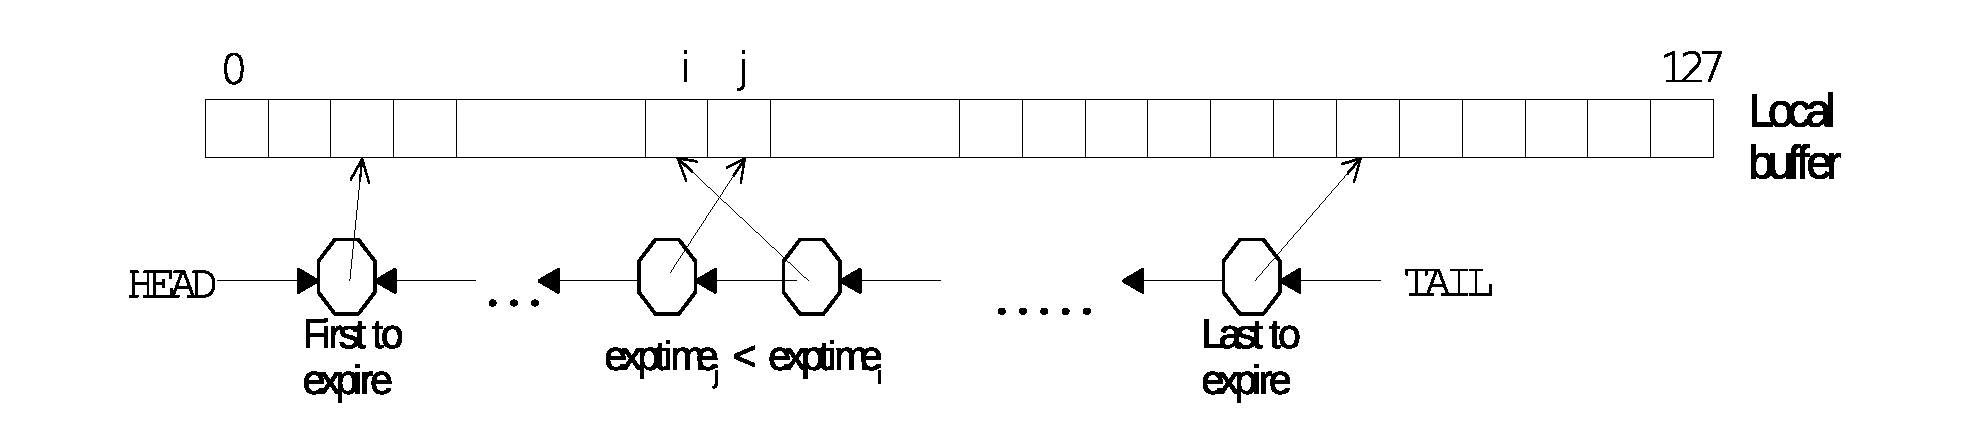
\includegraphics[scale=0.35]{images/queue}
\caption{Coda timeout}
\end{figure}
%
